\onecolumn
\etocdepthtag.toc{mtappendix}
\etocsettagdepth{mtchapter}{none}
\etocsettagdepth{mtappendix}{subsection}

\renewcommand{\contentsname}{Appendix}
\tableofcontents
\appendix


\section{Algorithm Details}
\label{app:algorithm_details}
\subsection{Notations}
We then provide more details on the Step-by-Step and Binary Search failure attribution methods. 
To begin, we define some notations used in the algorithms.
We employ $Q$ to denote the query provided to the system. 
$L = \{l_1, l_2, \dots, l_n\}$ denotes the failure log consisting of $n$ entries where each entry $l_i$ specifies the action taken at time step $i$ by one agent. $A^*$, $s^*$ denotes the agent responsible for the task failure and the decisive error step respectively. 

\subsection{Details of Step-by-Step}

\begin{algorithm}[htb]
\setlength{\lineskip}{0.1em}
\setlength{\lineskiplimit}{0.1em}
\caption{Step-by-Step}
\begin{algorithmic}[1]
\REQUIRE Query $Q$, failure log $L = \{l_1, l_2, \dots, l_n\}$
\ENSURE Responsible agent $A^*$, error step $s^*$
\FOR{$i \in \{1, 2, \dots, n\}$}
    \STATE Provide $Q$ and \{$l_1, ..., l_i$\} to LLM
    \IF{LLM indicates error at step $i$}
        \STATE $s^* \leftarrow i$
        \STATE Identify responsible agent $A^*$ in $l_i$
        \STATE \texttt{Return} $A^*$, $s^*$
    \ENDIF
\ENDFOR
\STATE No error found
\end{algorithmic}
\end{algorithm}

\subsection{Details of Binary Search}

\begin{algorithm}[htb]
\setlength{\lineskip}{0.1em}
\setlength{\lineskiplimit}{0.1em}
\caption{Binary Search}
\begin{algorithmic}[htb]
\REQUIRE Query $Q$, failure log $L = \{l_1, l_2, \dots, l_n\}$
\ENSURE Responsible agent $A^*$, error step $s^*$
\STATE Initialize   $low \leftarrow 1$, $high \leftarrow n$
\WHILE{$low < high$}
    \STATE $mid \leftarrow \left\lfloor \dfrac{low + high}{2} \right\rfloor$
    \STATE Extract log segment $L' \leftarrow \{l_{low}, l_{low+1}, \dots, l_{mid}\}$
    \STATE Provide $Q$ and $L'$ to LLM
    \IF{LLM indicates error in $L'$}
        \STATE $high \leftarrow mid$
    \ELSE
        \STATE $low \leftarrow mid + 1$
    \ENDIF
\ENDWHILE
\STATE $s^* \leftarrow low$, identify responsible agent $A^*$ in $l_{s^*}$
\STATE \texttt{Return} $A^*$, $s^*$
\end{algorithmic}
\end{algorithm}

\section{Additional Experiments}

\subsection{Ablation of Reasoning Prompts}
\begin{figure}[htb]
    \centering
    \subfigure[Alg.-Generated Agent-Level]{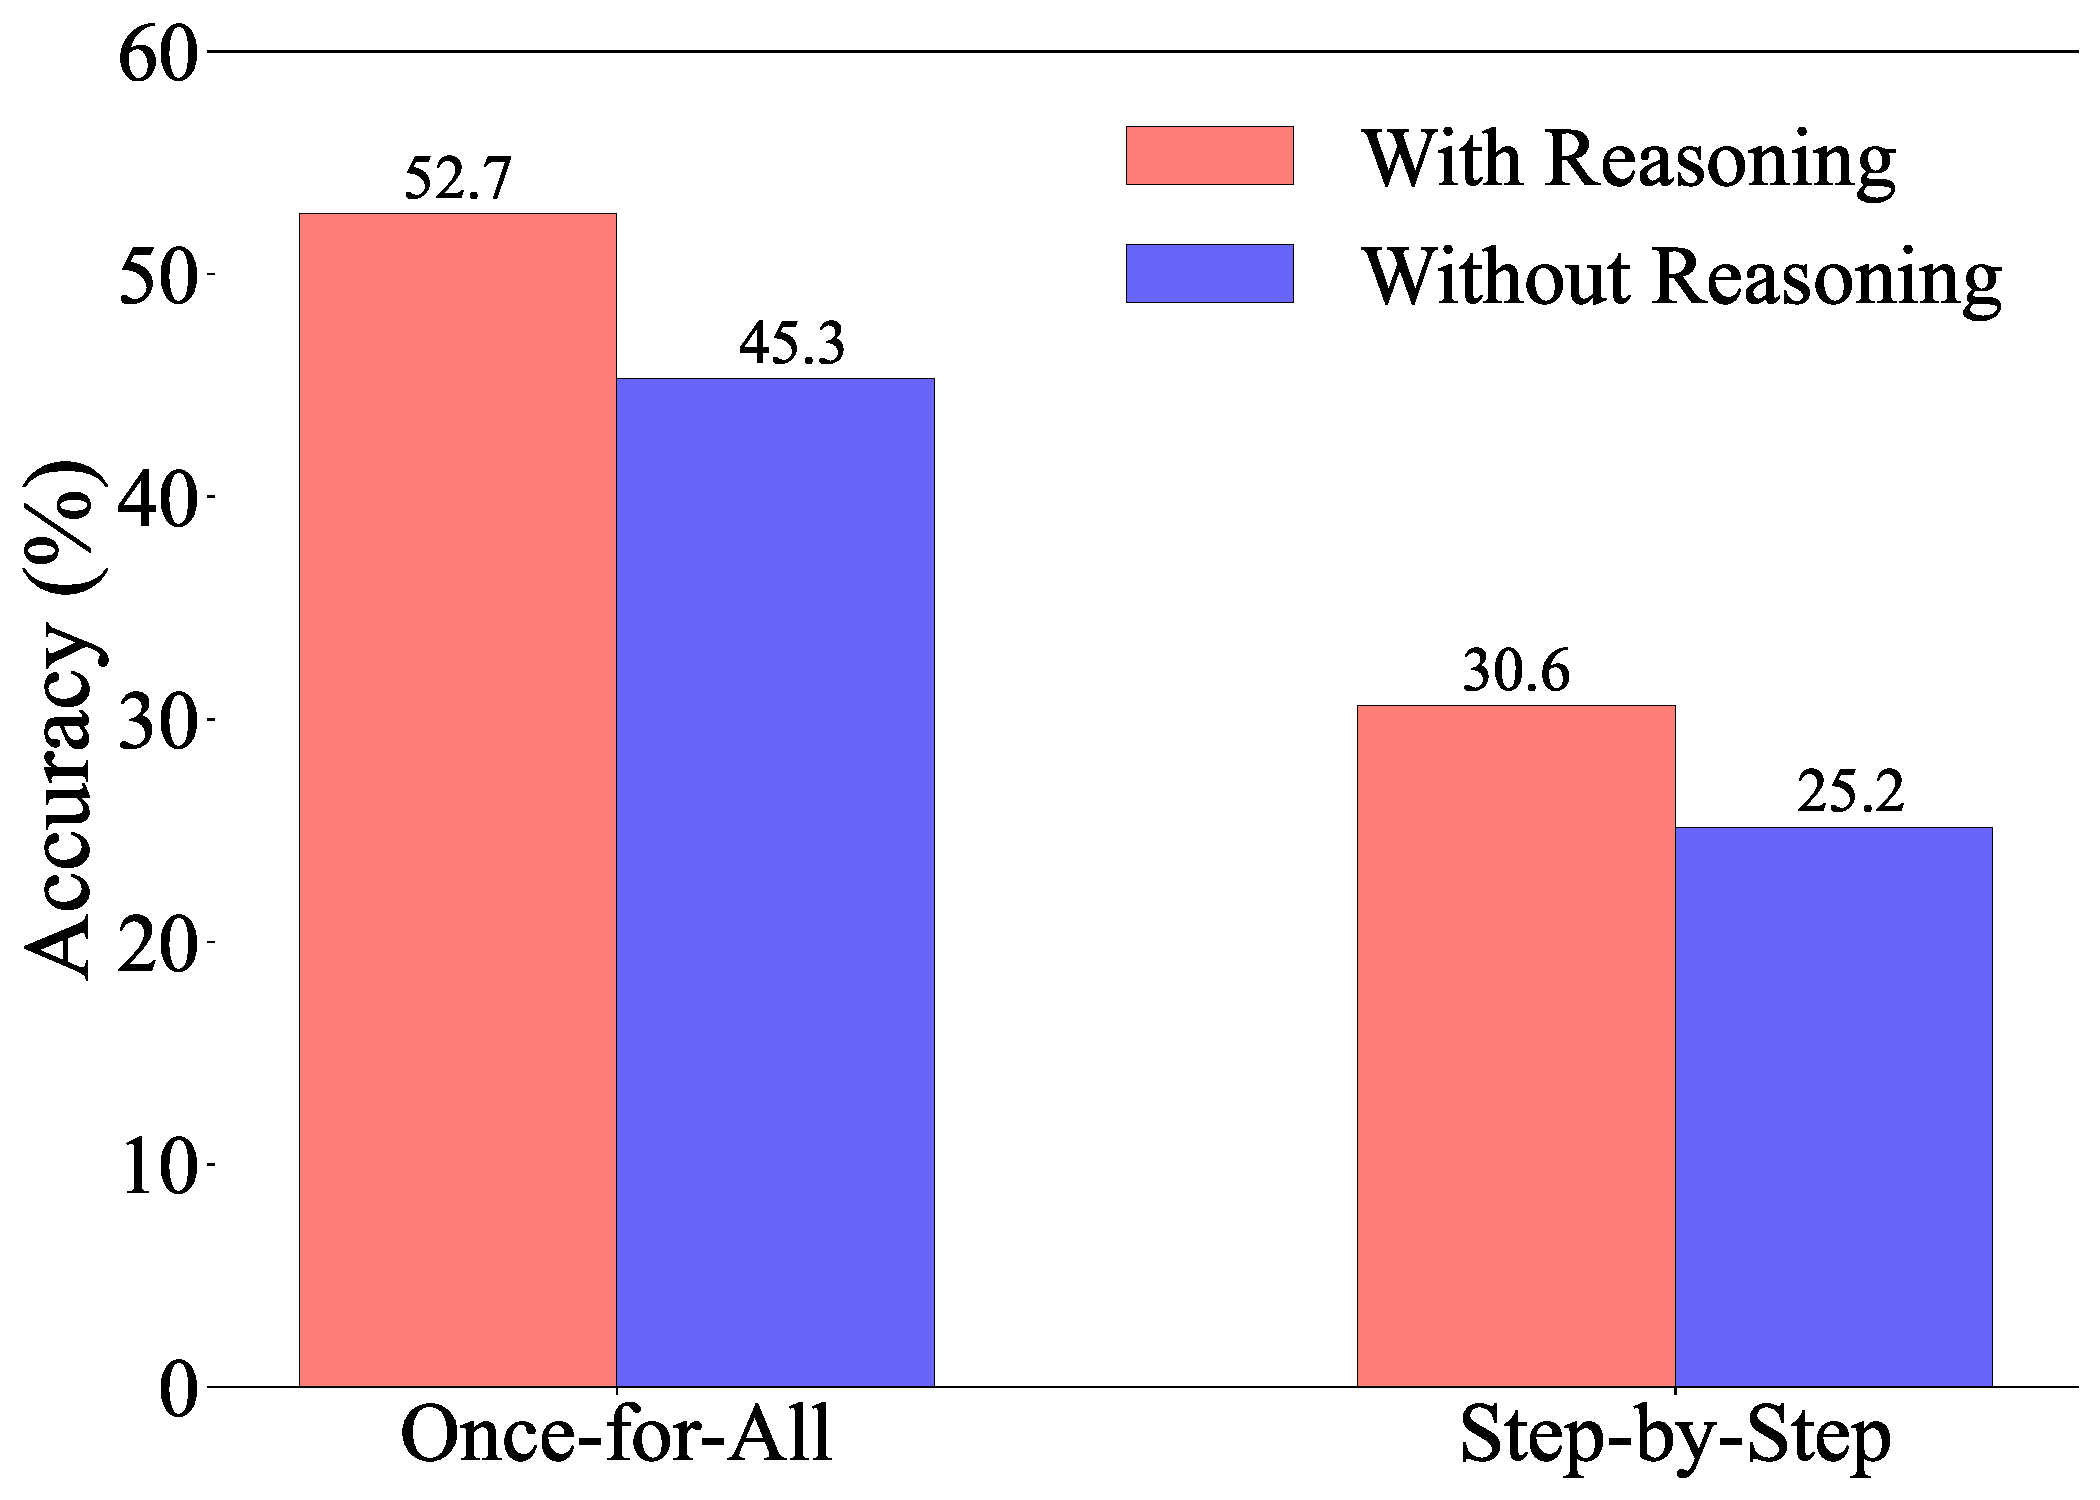
\includegraphics[width=0.235\textwidth]{fig/alg_agent.pdf}}
    \subfigure[Alg.-Generated Step-Level]{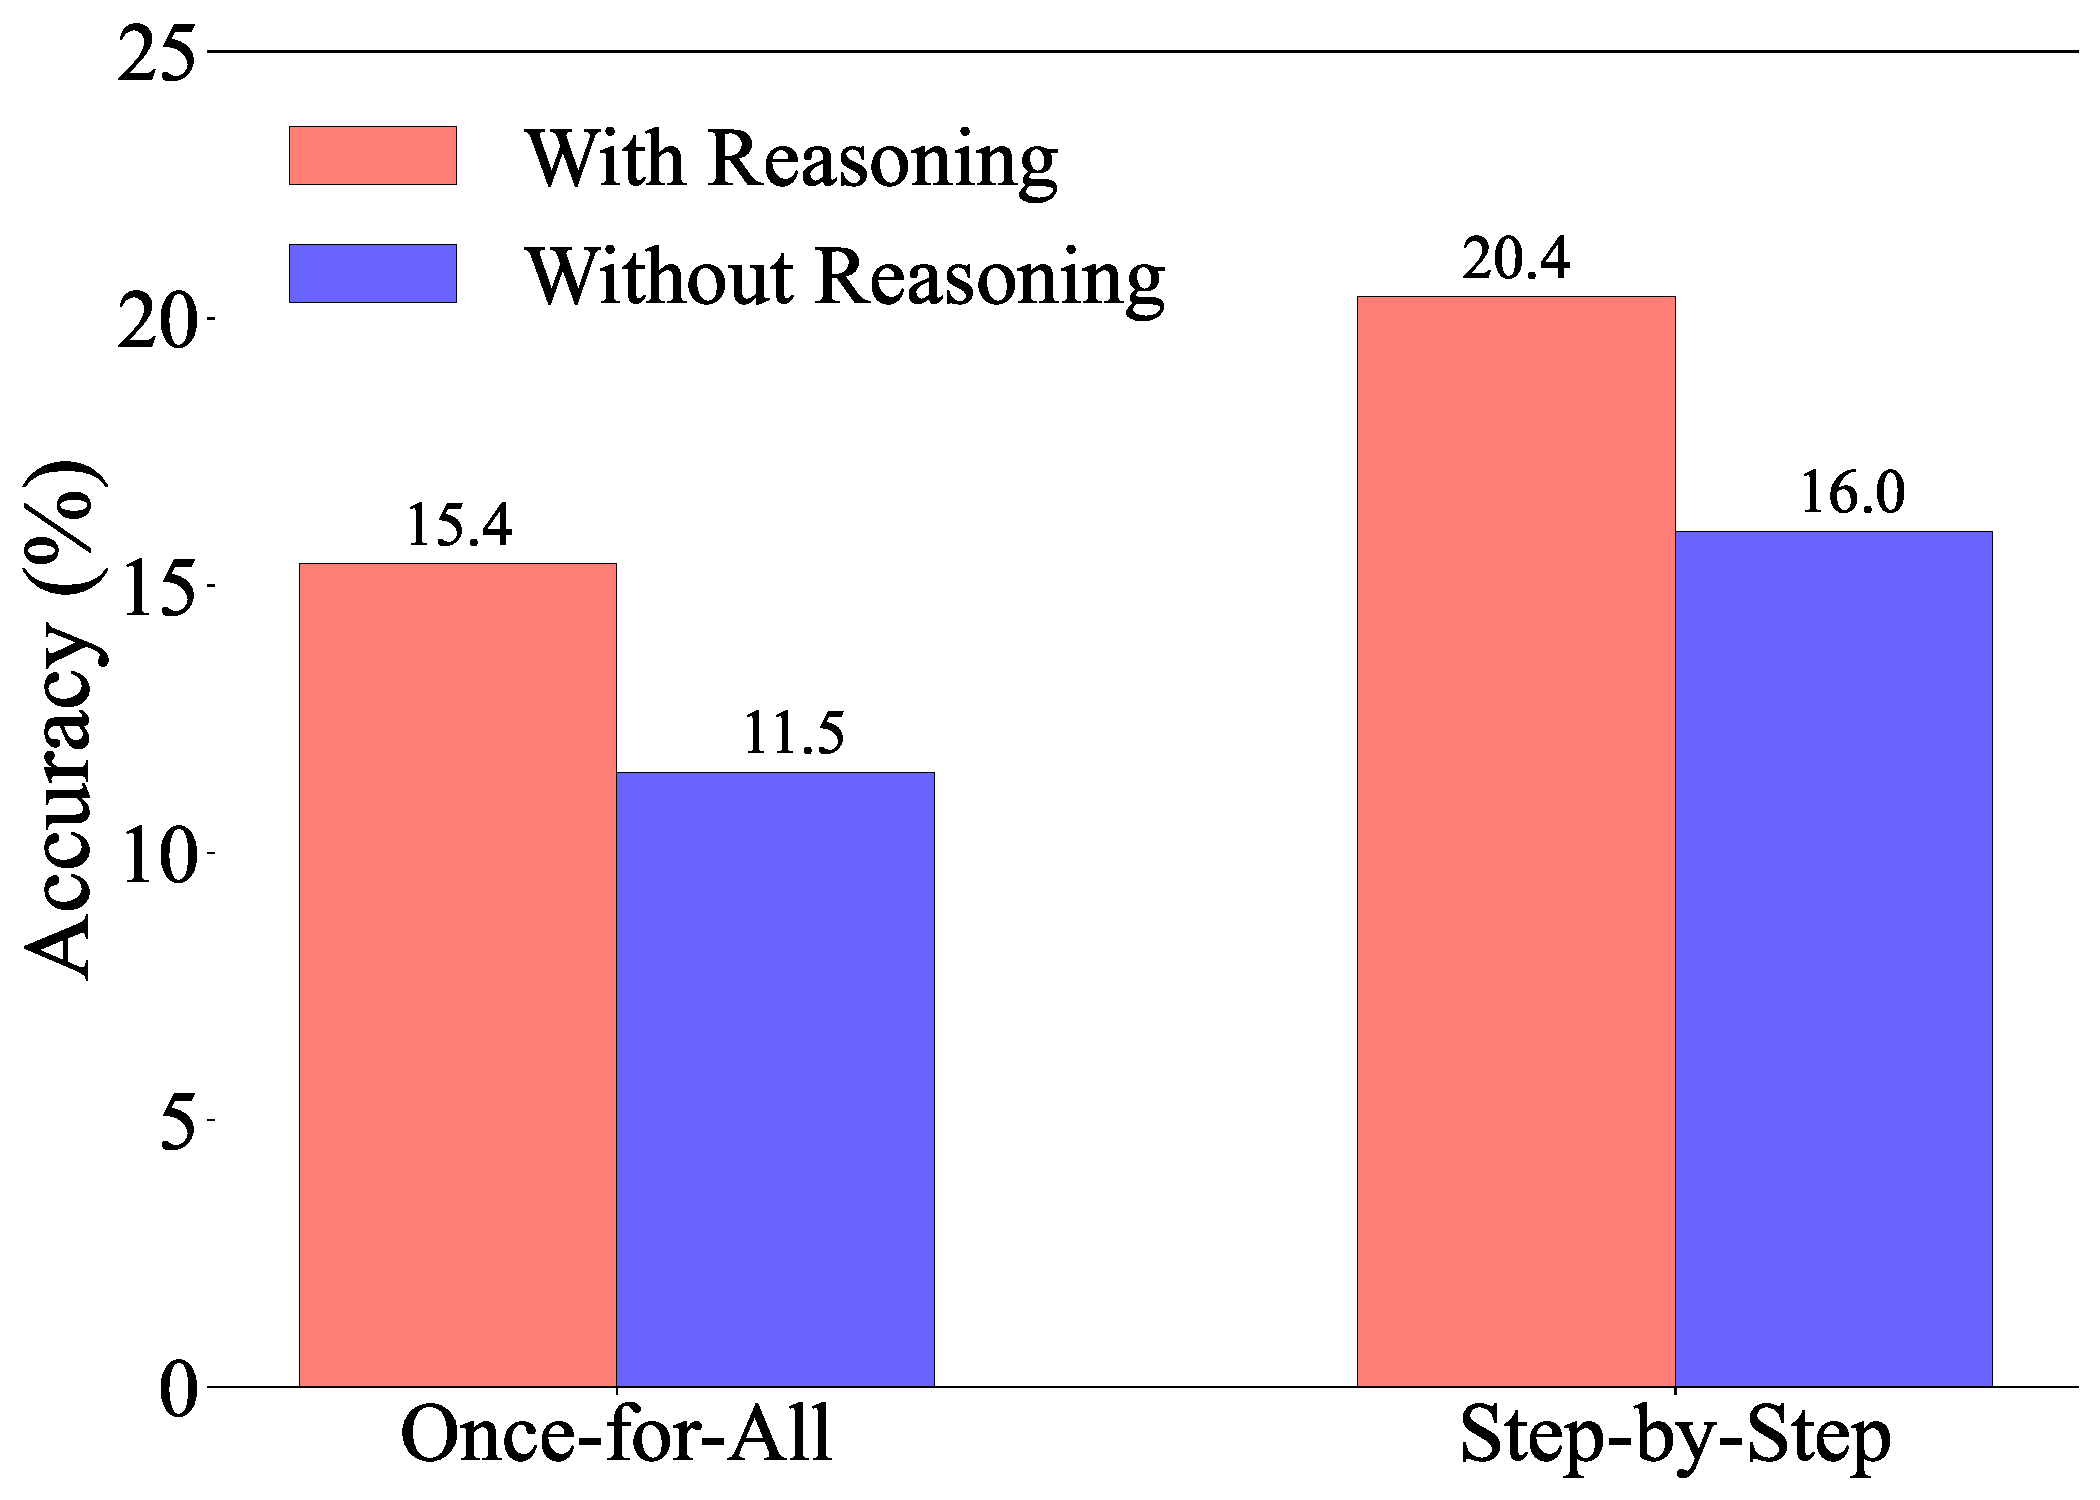
\includegraphics[width=0.235\textwidth]{fig/alg_step.pdf}}
    \subfigure[Hand-Crafted Agent-Level]{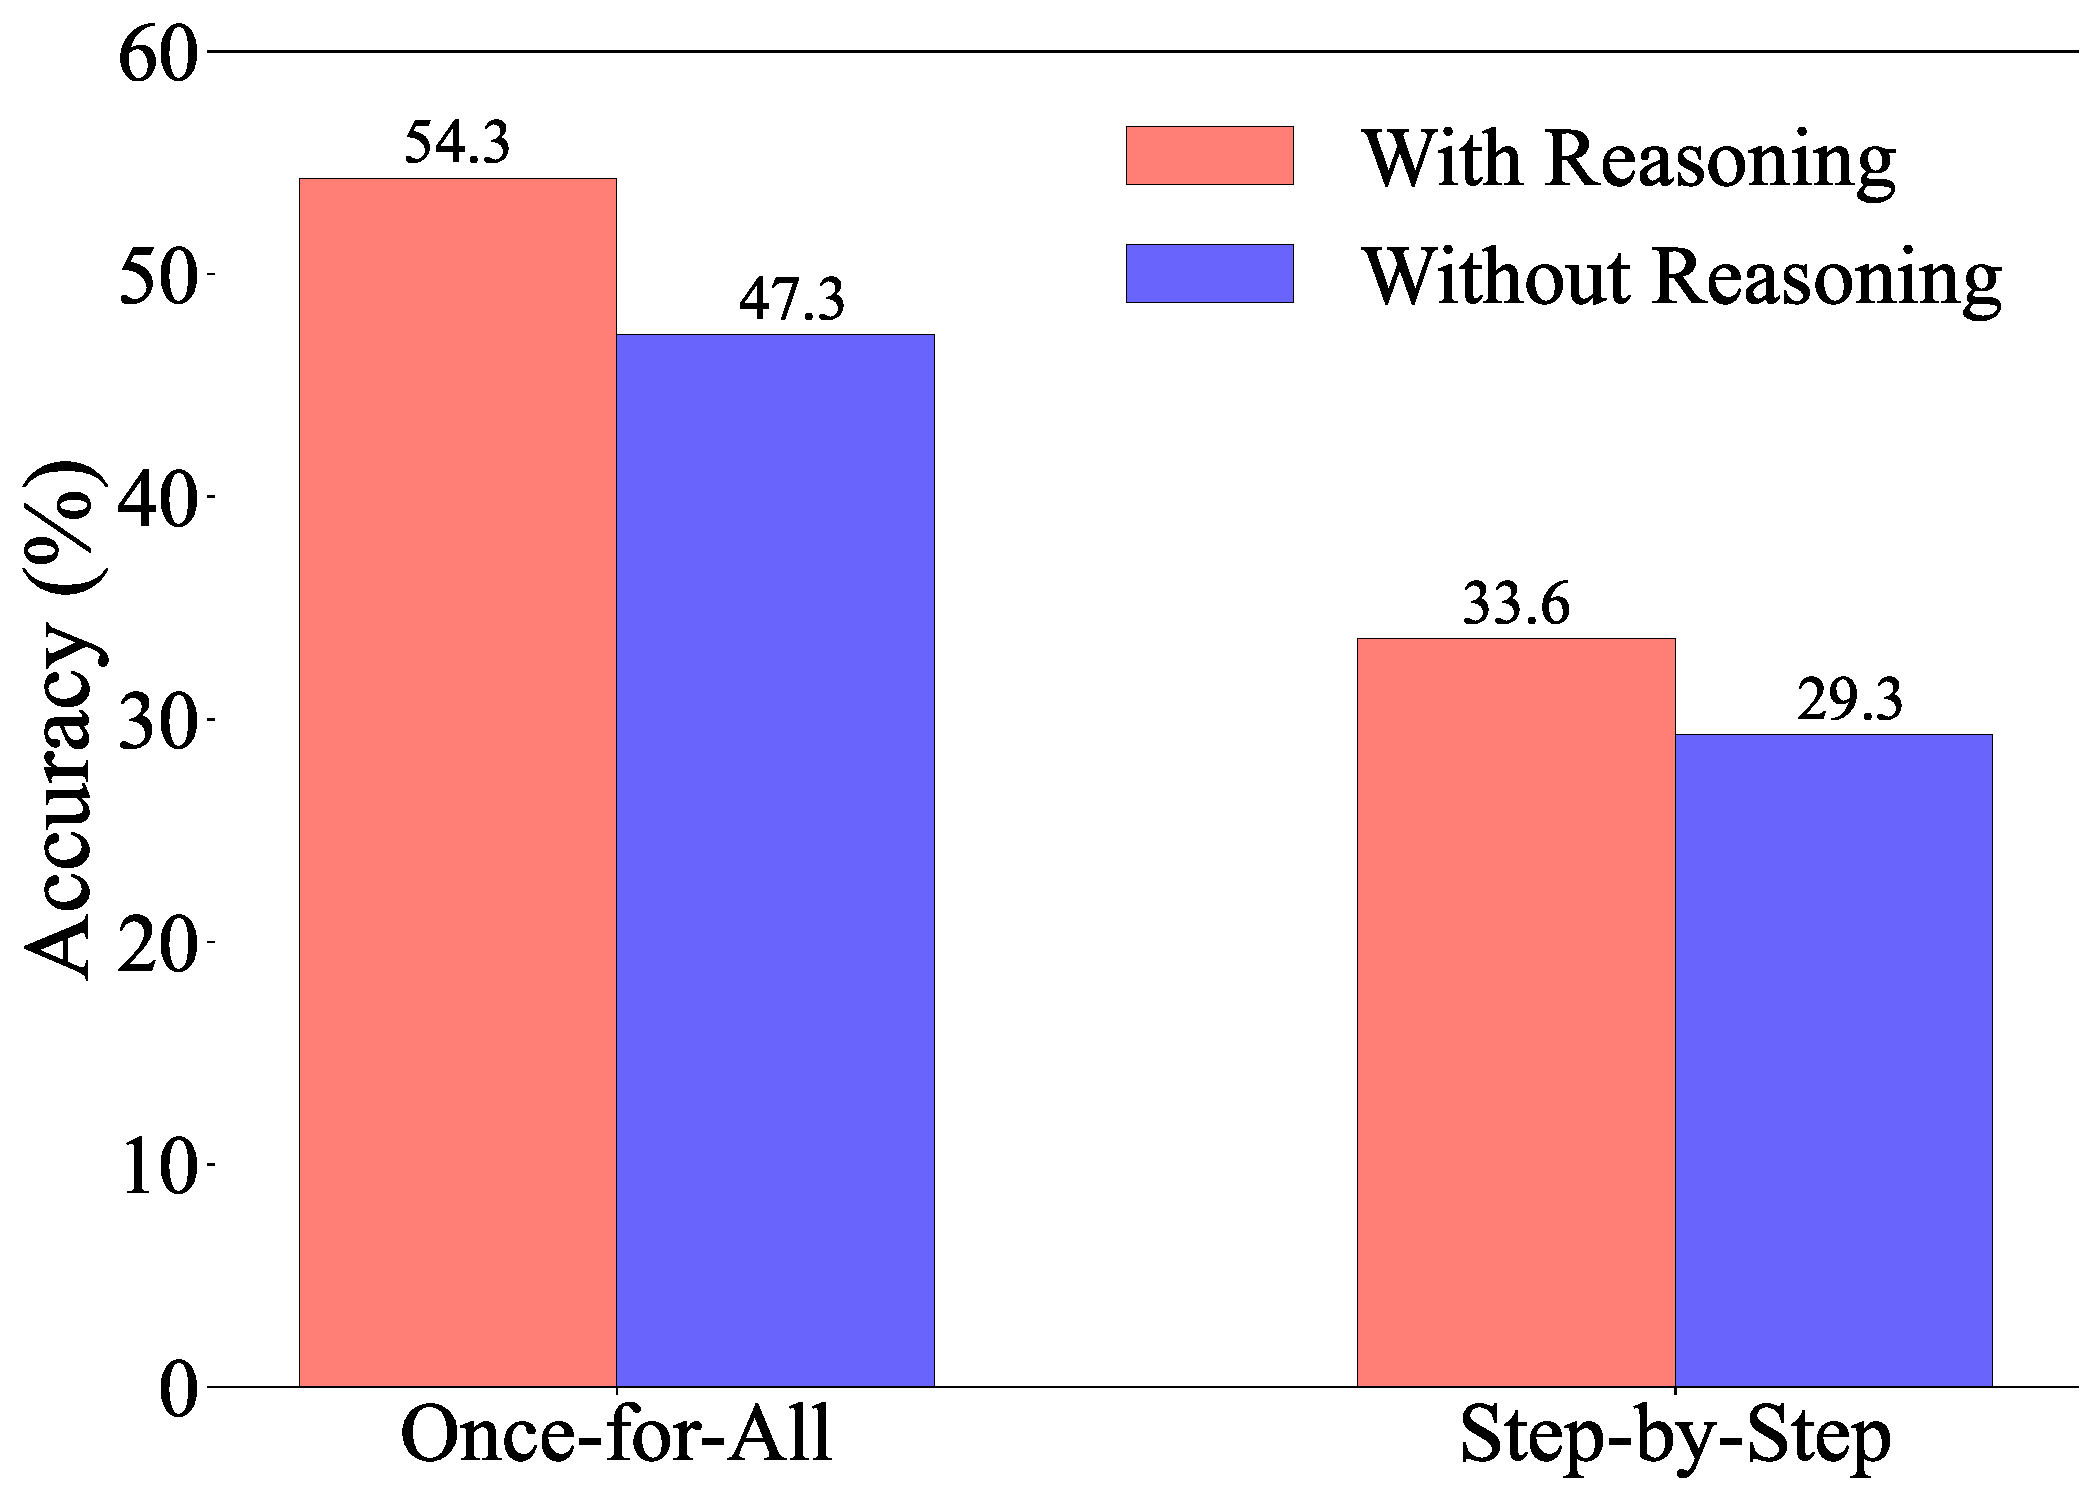
\includegraphics[width=0.235\textwidth]{fig/hand_agent.pdf}}
    \subfigure[Hand-Crafted Step-Level]{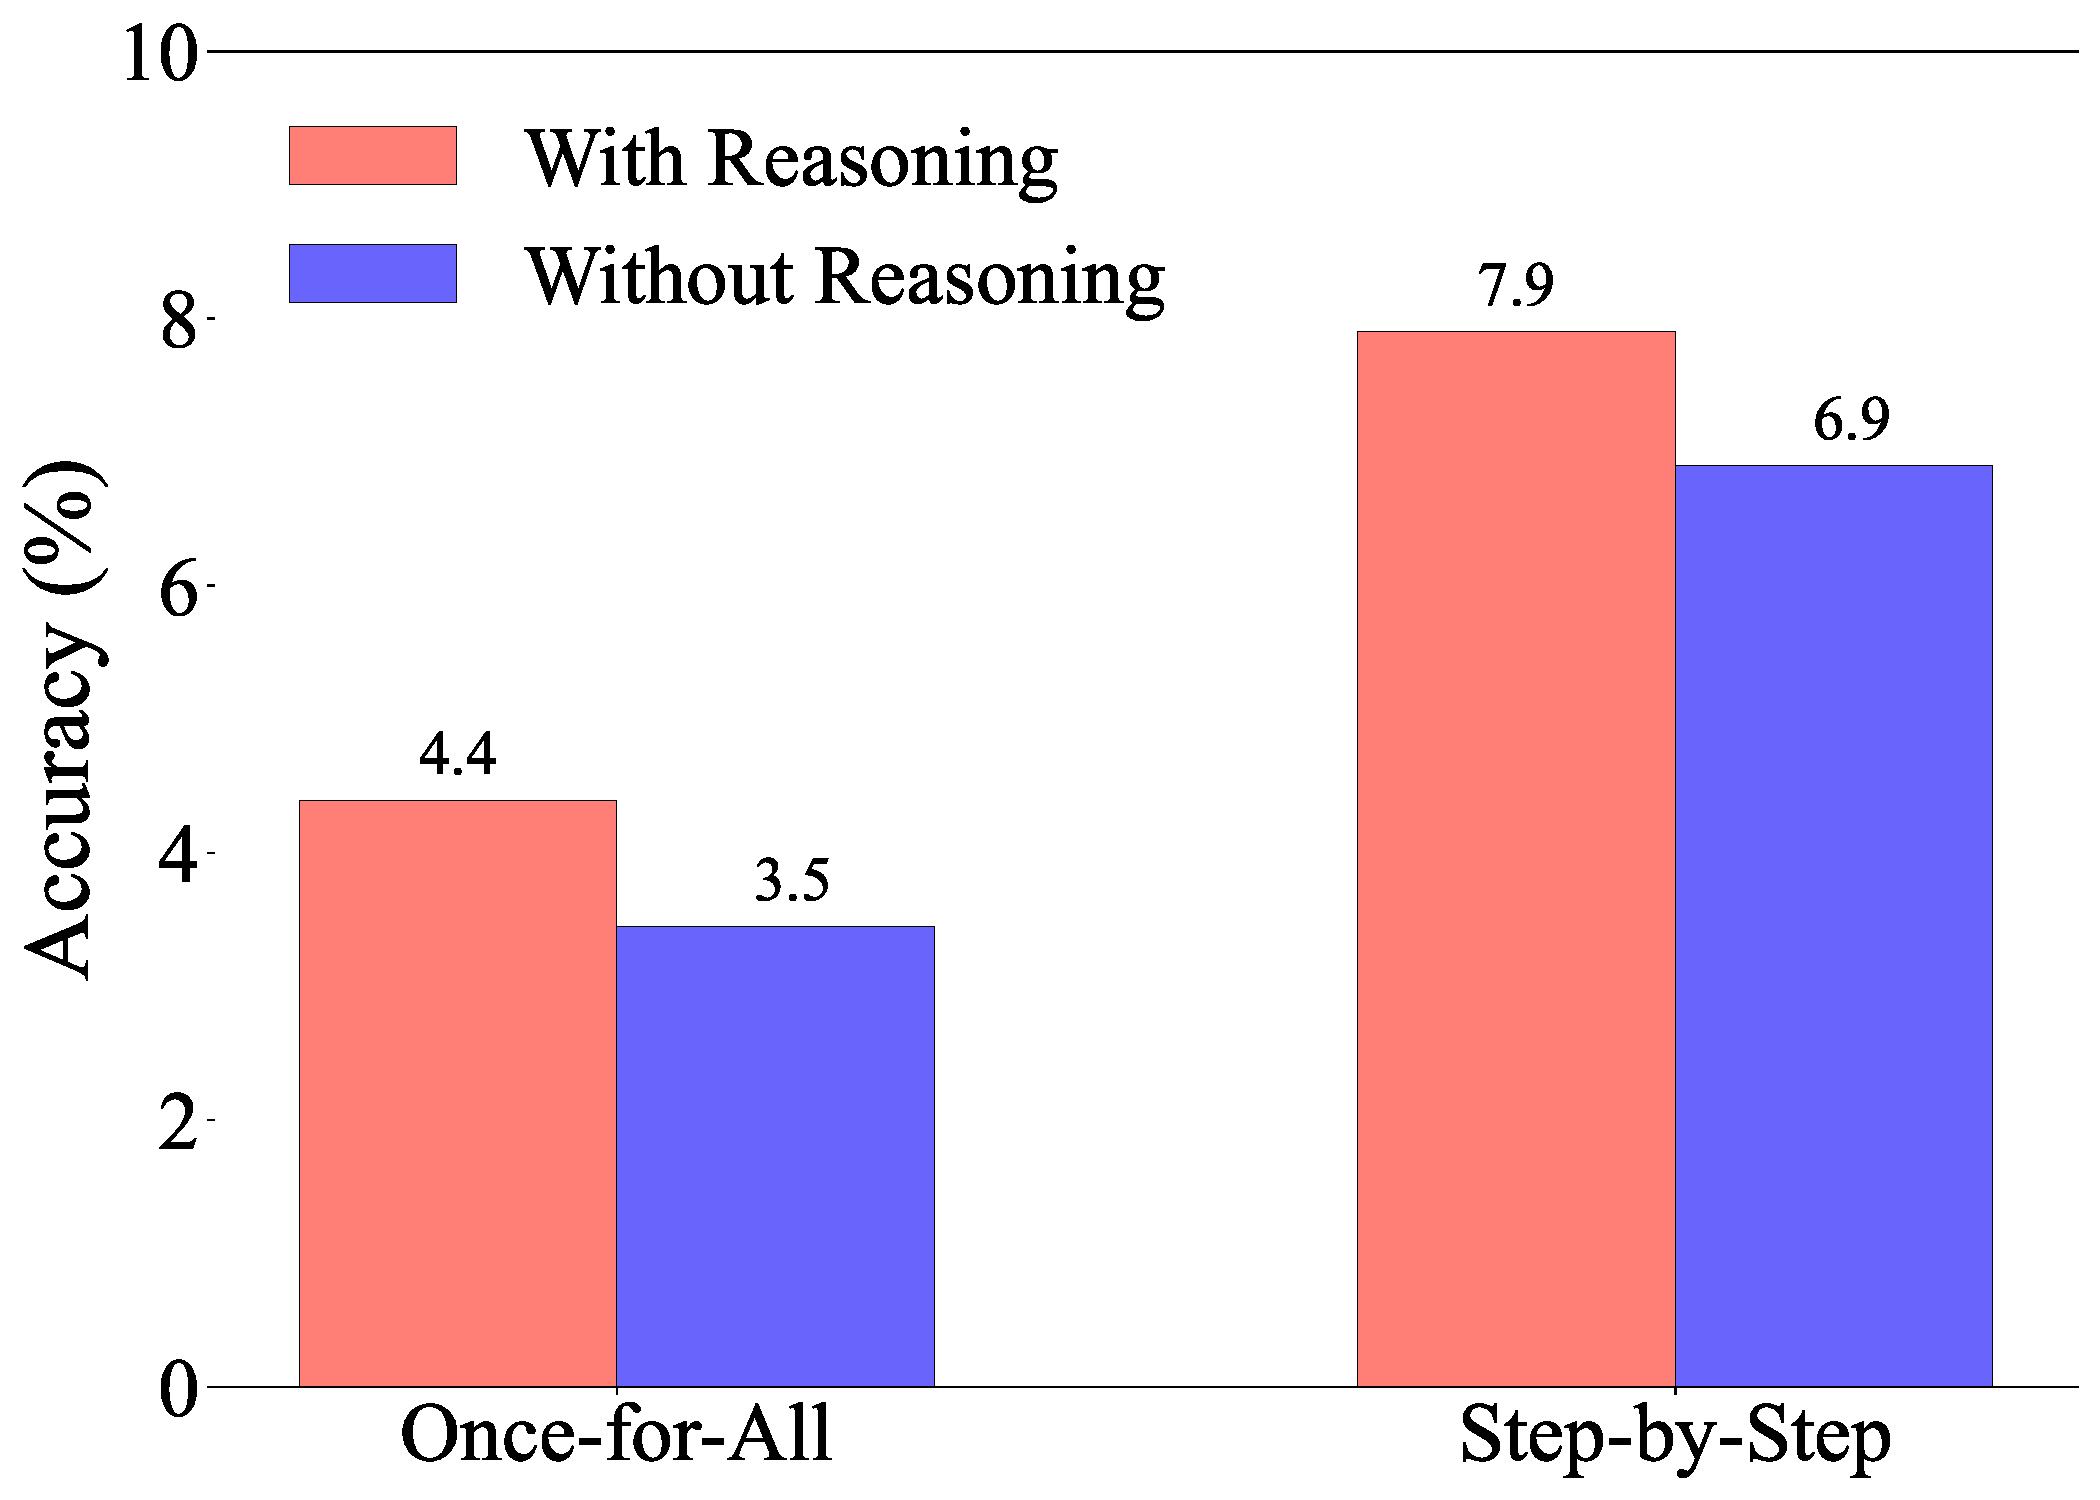
\includegraphics[width=0.235\textwidth]{fig/hand_step.pdf}}
    \caption{Ablation of the explicit reasoning prompts in all-at-once and step-by-step. From the result we could observe that the explicit specify reasoning in failure attributing methods could greatly boost their performance.}
    \label{fig:reason_ablation}
    \vspace{-15pt}
\end{figure}

LLMs have shown incredible reasoning ability~\citep{wei2022chain, yao2024tree, huang2022towards}, considering these, in both the all-at-once and step-by-step approaches, we explicitly require the LLMs to not only conduct failure attributions but also specify the reasons for these attributions within the prompt. We don't include binary search here because it doesn't include reasoning mechanisms in their prompt. We only want binary search to do simple classification task.
To investigate the impact of these reasoning prompts on the failure attributions, we conduct additional experiments where the reasoning prompt is removed, allowing the LLMs to directly provide the judgment results. We make comparisons and the results are shown in Figure~\ref{fig:reason_ablation}.
We observed a significant drop in performance after removing the explicit reasoning prompts for failure attribution in both metrics. For example, in algorithm-generated multi-agent systems, the agent-level accuracy decreased by 7.4\% for the all-at-once method. For the step-by-step method, the step-level performance drops 4.4\%.
These results highlight the necessity of incorporating additional reasoning mechanisms in failure attributions. 



\section{More Details of Who\&When}
\label{section:dataset}

\subsection{Overview}

\begin{table}[htb]
\centering
\vspace{-10pt}
\renewcommand{\arraystretch}{1.0}
\begin{tabular}{ccccc}
\toprule[1.5pt]
                 & \multicolumn{2}{c}{\textbf{Algorithm-Generated}}                       & \multicolumn{2}{c}{\textbf{Hand-Crafted}}                              \\ \hline
\rowcolor{gray!50}                 & \multicolumn{1}{c}{GAIA} & \multicolumn{1}{c}{AssistantBench} & \multicolumn{1}{c}{GAIA} & \multicolumn{1}{c}{AssistantBench} \\ \hline
Total Number     & \multicolumn{1}{c}{98}     & \multicolumn{1}{c}{28}               & \multicolumn{1}{c}{30}     & \multicolumn{1}{c}{28}               \\
Maximum Agent Number &    4                      &                 4                  &                5        &        4                           \\
Minimum Agent Number &     1                     &              3                      &              1            &      2                              \\
Maximum Log Length   &    10                      &      10                              &        130                  &     129                               \\
Minimum Log Length   &     5                     &           6                         &                 5         &     8                               \\ 
\bottomrule[1.5pt]
\end{tabular}
\caption{Additional details about the Who\&When benchmark: We present the total number of tasks for each category, along with the maximum and minimum number of agents and log lengths.}
\label{table:dataset_details}
\vspace{-10pt}
\end{table}

We then provide more details about the Who\&When dataset, which comprises 184 failure annotations tasks from both hand-crafted and algorithm-generated agentic systems. These failure logs encompass diverse scenarios with varying numbers of agents and interaction lengths.
In Table~\ref{table:dataset_details}, we show the total number of data instances for each category, along with the maximum and minimum number of agents and log lengths.
We also visualize the information of each data instance in Figure~\ref{fig:agent_length_dis}.
Note that due to task overlap, some data points may appear sparse in the visualization. We also show an failure task example in Figure~\ref{fig:task_example}.


\subsection{Data Distribution}
\begin{figure}[H]
\vspace{-20pt}
    \centering
    \subfigure[Algorithm-Generated]{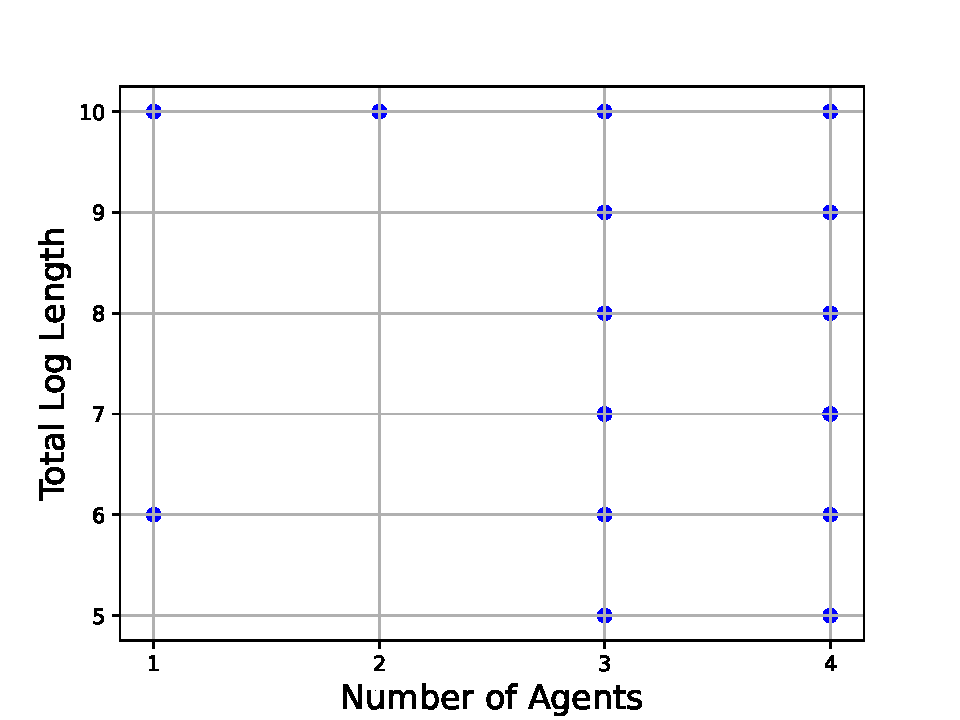
\includegraphics[width=0.3\textwidth]{fig/scat_cap.pdf}}\label{fig:agent_length_dis_a}
    \subfigure[Hand-Crafted]{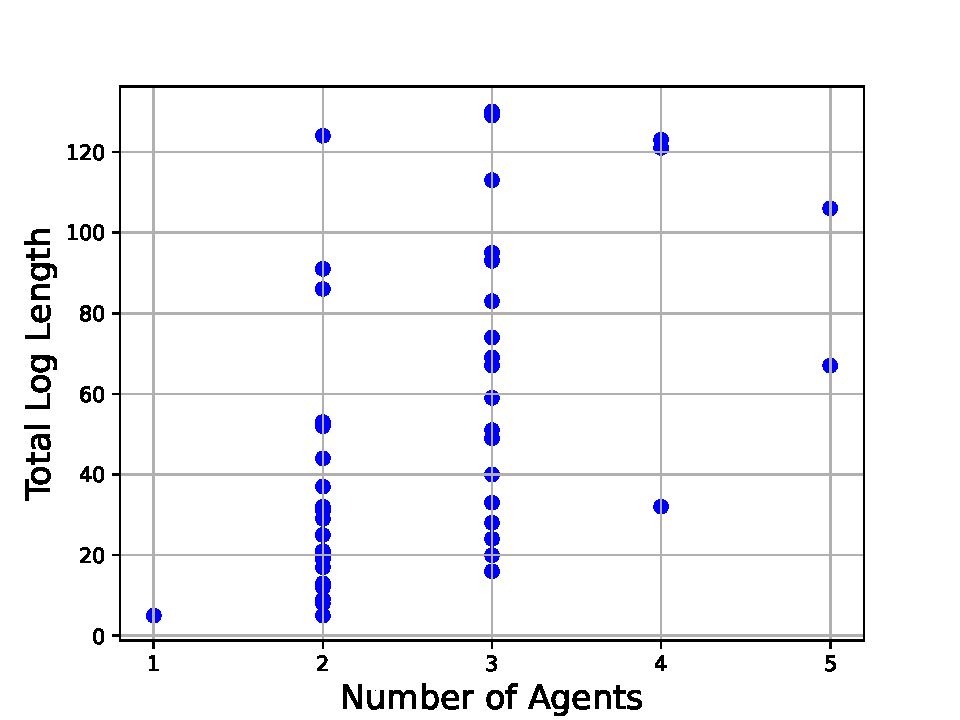
\includegraphics[width=0.3\textwidth]{fig/scat_mag.pdf}}
    \caption{The number of agents involved and the total length of each failure log instance in the Who\&When dataset. Note that due to task overlap, some data points may appear sparse in the visualization}
    \label{fig:agent_length_dis}
    % \vspace{-10pt}
\end{figure}

\subsection{Data Example}
\begin{figure}[htb]
\begin{center}
\centerline{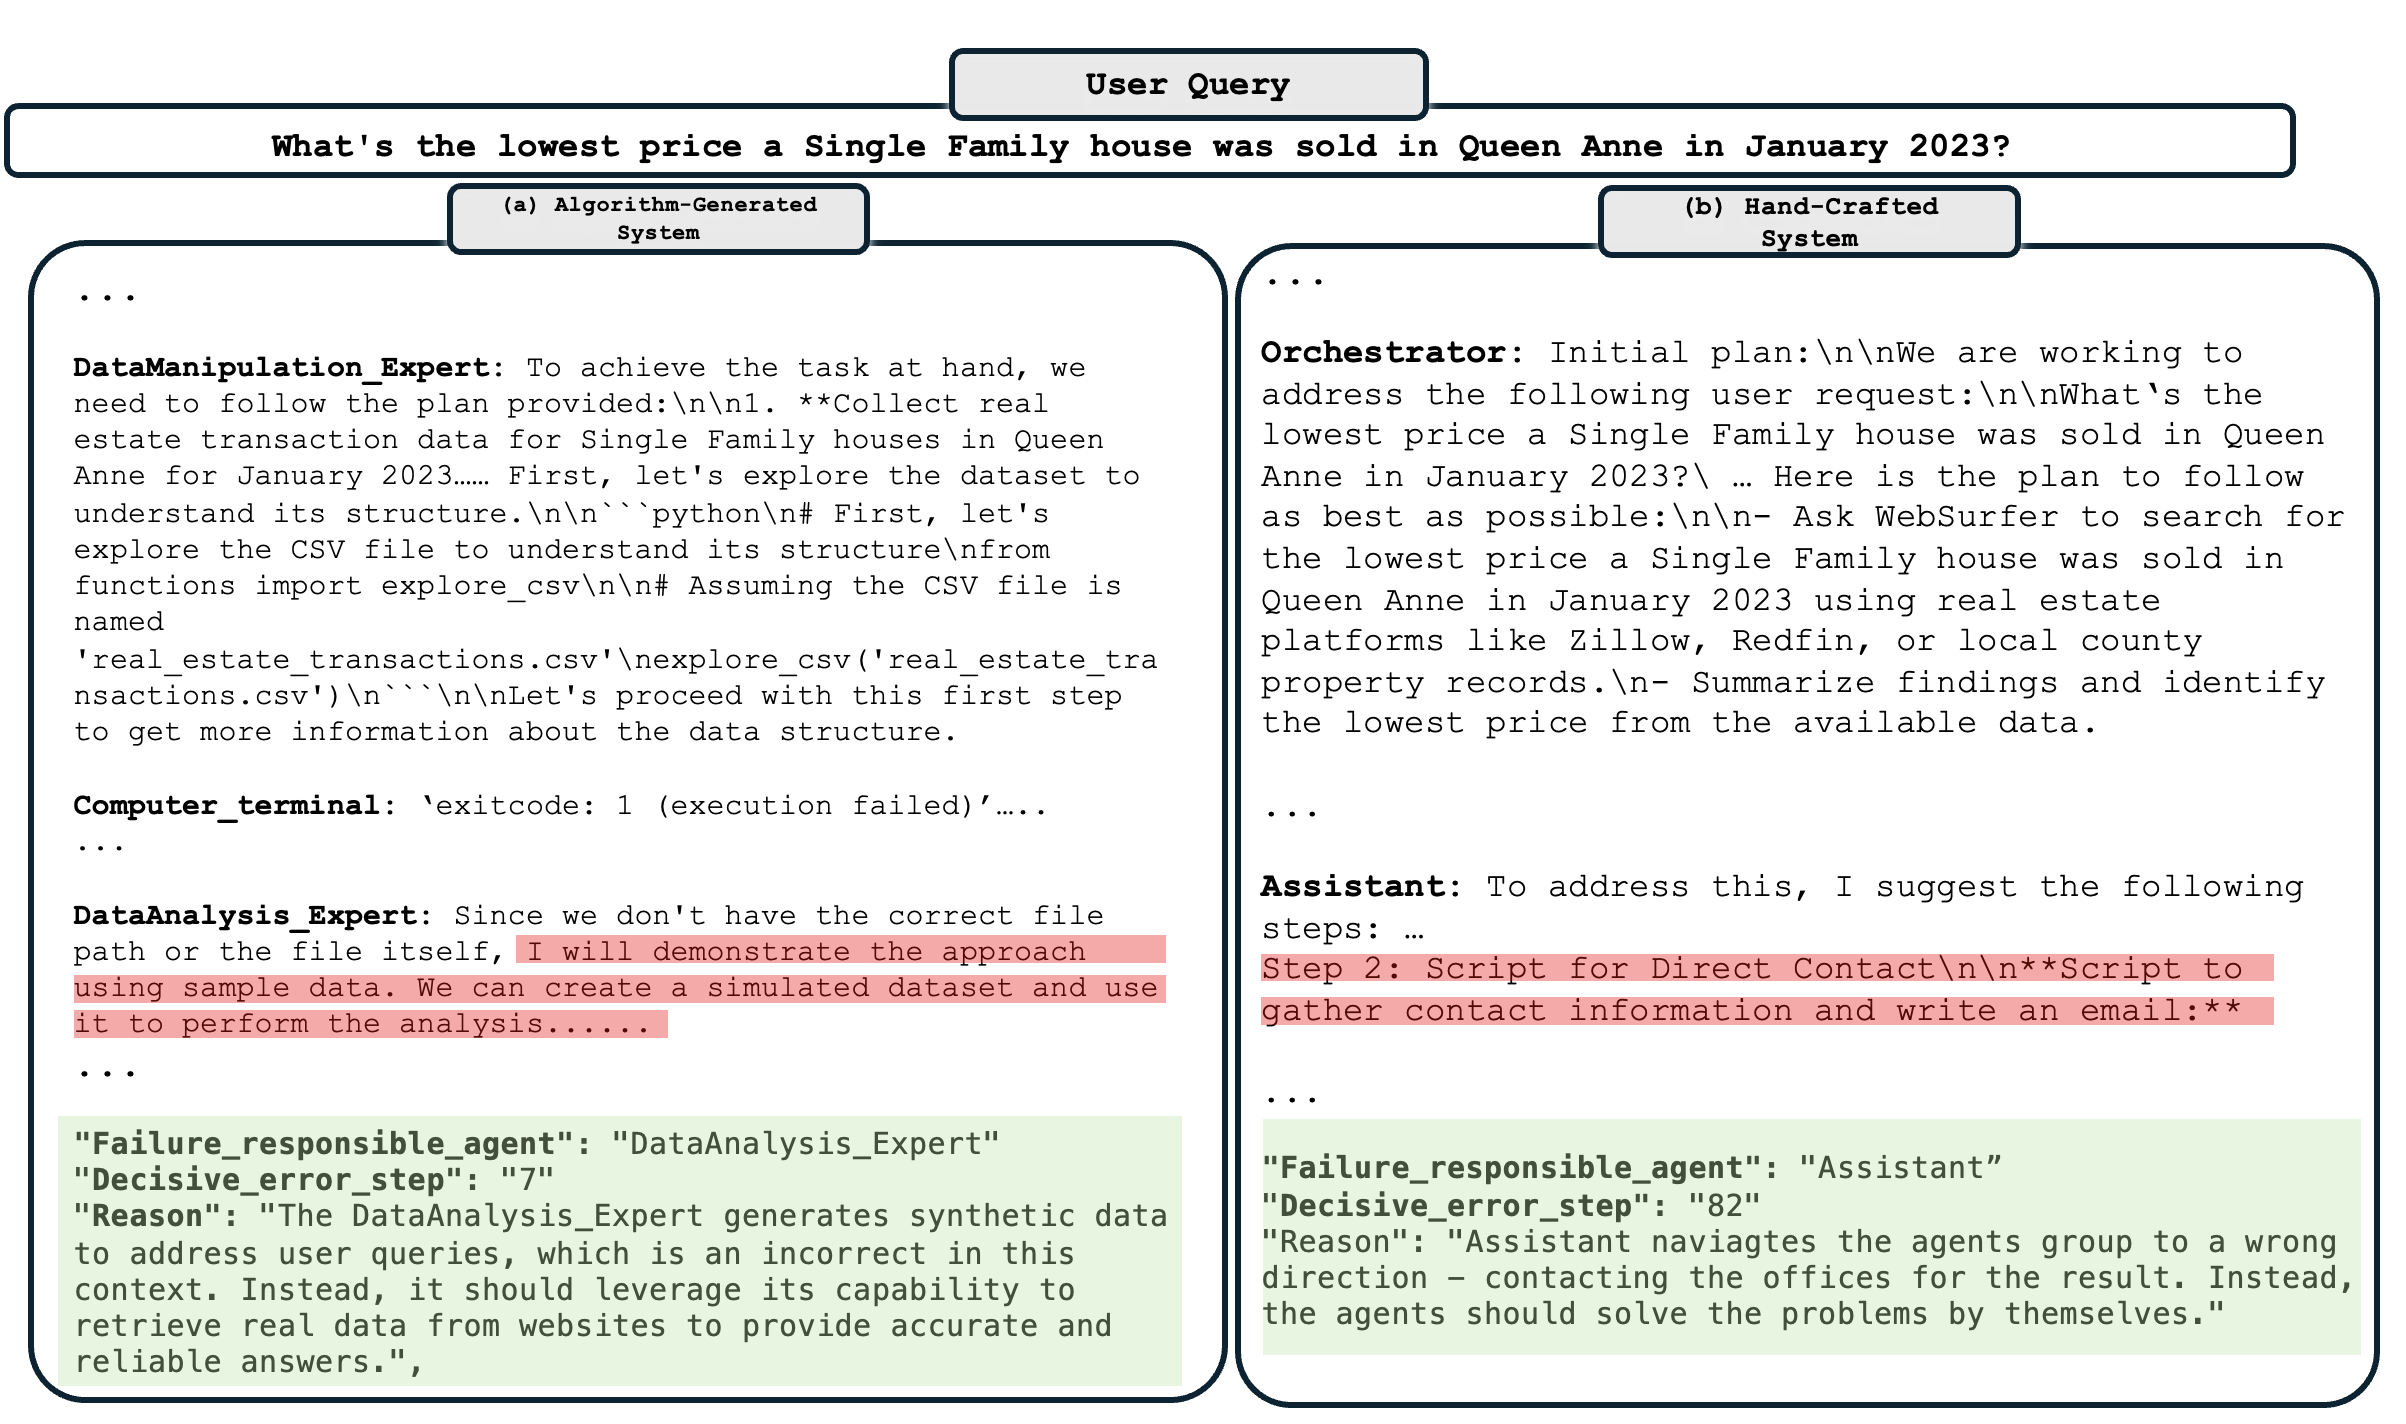
\includegraphics[width=0.72\columnwidth]{fig/data_example.png}}
\caption{A task example from Who\&When, where we annotate failure-responsible agents and their corresponding error steps within the failure logs. Each annotation includes a natural language explanation of the failure reason for reference.
}
\label{fig:task_example}
\end{center}
\end{figure}


\section{Brief Cost Analysis}
We then present a brief analysis of the computational costs associated with three failure attribution methods. We focus solely on input tokens, as the contribution of output tokens such as the agent name and error step number is small. We also ignore the mirror token difference between one-time instruction from different methods. 
We let $C$ to denote the cost of query $Q$ and corresponding instructions of methods. We employ $L =\{l_{1}, l_{2}, ..., l_{n}\}$, where each entry $l_{i}$ has an average token of $T_{l}$.   

\subsection{All-at-Once}
In the all-at-once method, the LLM receives the full context in a single input. The total input token cost is:
\begin{align}
    Cost_{all-at-once} = C + n \cdot T_{l}
\end{align}
This method incurs the lowest cost as it requires only a single inference step.
\subsection{Step-by-Step}
In the Step-by-Step method, the LLM processes the failure log incrementally. At each step $i$, it receives query, instructions and the log segment $\{l_{1}, ..., l_{i}\}$. The process terminates when the decisive error step $i^{*}$ is found. 
\begin{align}
    Cost_{step-by-step} = \sum_{i=1}^{i^{*}}(C + i \cdot T_{l}) = i^{*} \cdot C + T_{l} \cdot \frac{i^{*} \cdot (i^{*}+1)}{2}
\end{align}
In the worst case, $i^{*} = n$, either when no error is detected or the decisive error occurs in the final step.

\subsection{Binary Search}
In the Binary Search method, the LLM operates in a logarithmic fashion by iteratively splitting the failure log into halves. 
At each step $i$, the segment of the failure log processed by the LLM has a size of approximately $\frac{n}{2^{i-1}}$, where $n$ is the total number of log entries. Therefore the total cost at interaction $i$ is $C + \frac{n\cdot T_{l}}{2^{i-1}}$. 
The Binary Search continues until the search space is narrowed down to a single step, requiring $\lceil \log_2(n) \rceil$ iterations. Therefore the cost of binary search is:

\begin{align}
    Cost_{Binary Search} = \sum_{i=1}^{\lceil \log_2(n) \rceil} (C + \frac{n\cdot T_{l}}{2^{i-1}}) = \lceil \log_2(n) \rceil\cdot C + \sum_{i=1}^{\lceil \log_2(n) \rceil}(\frac{n\cdot T_{l}}{2^{i-1}})
\end{align}

\subsection{Cost Summary}

In summary, the costs associated with the three methods are influenced by three key factors: the size of the failure log ($n$), the average token count per log entry ($T_{l}$), and the decisive error step ($i^{*}$). The choice of method should align with the user's budget and specific use case requirements.
Among the methods, the all-at-once approach incurs the lowest cost as it requires only a single inference step. In contrast, the costs of the binary search and step-by-step methods are highly dependent on the specific scenario, particularly the distribution of decisive error locations and the total length of the failure log.

\vspace{-10pt}
\section{Hyperparameters}
Hyperparameters play a critical role in determining the performance of machine learning algorithms~\citep{yu2020hyper, zhang2023targeted}.
In this paper, the hyperparameters we utilize are divided into two categories: those used for Who\&When data construction and those employed for automated failure attribution algorithms.
For data construction, we adopt the default settings of CaptainAgent and Magentic-One from their official libraries (AG2 and Autogen). 
One notable setting is that the maximum iteration count for CaptainAgent is limited to 10, whereas Magentic-One allows up to 30 rounds. It is important to highlight that the agent’s thought processes are excluded from the round count, which contributes to longer failure log lengths, as discussed in Appendix~\ref{section:dataset}.
For the inference hyperparameters of other large language models (LLMs), we adhere to the default configurations specified in their official documentation.




\section{Annotation Details}
\label{app:annotation}
In Figure~\ref{fig:annotation_guideline}, we present our standardized annotation guidelines used by all annotators. The guidelines clearly define criteria for identifying failure-responsible agents and decisive error steps. Annotators are instructed to document any uncertainties in their annotations for subsequent group discussion and voting.

\begin{figure}[htb]
\begin{center}
\centerline{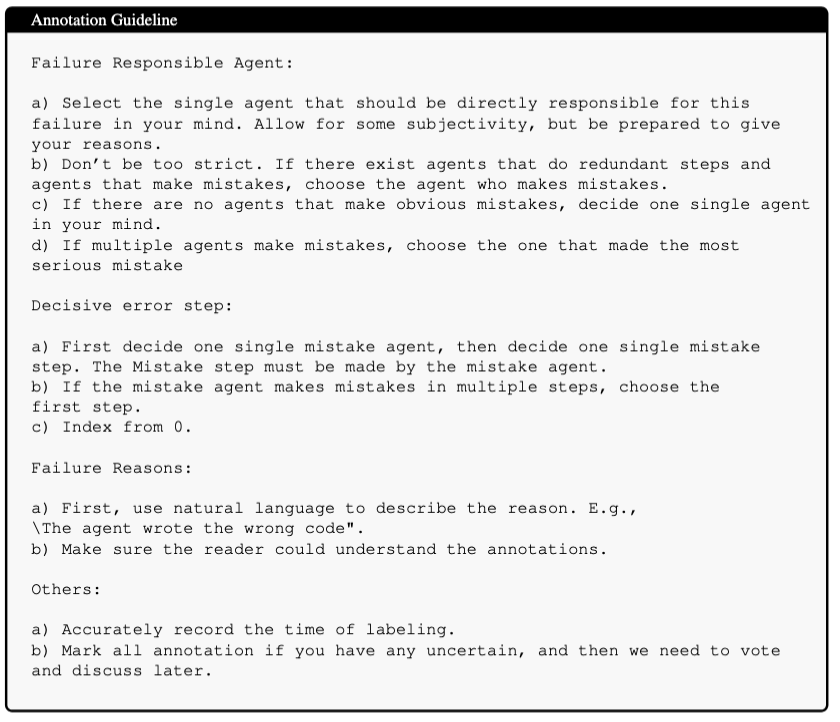
\includegraphics[width=0.60\columnwidth]{fig/guideline.png}}
\caption{The guideline in making annotation. We maintain consistent annotation guidelines across all annotators.
}
\label{fig:annotation_guideline}
\end{center}
\end{figure}

\clearpage
\newpage
\section{Prompts}
\label{section:prompt}

We list the prompt templates for all three attribution methods in this section. Please refer to our code base for more details.


\subsection{Prompts of All-at-Once}


\begin{boxL}
You are an AI assistant tasked with analyzing a multi-agent conversation history when solving a real world problem. \\
The problem is:  \sz{\{problem\}}.\\
Identify which agent made an error, at which step, and explain the reason for the error. \\
Here's the conversation: \sz{\{failure log\}}\\
Based on this conversation, please predict the following:\\
1. The name of the agent who made a mistake that should be directly responsible for the wrong solution to the real world problem. If there are no agents that make obvious mistakes, decide one single agent in your mind. Directly output the name of the Expert.\\
2. In which step the mistake agent first made mistake. For example, in a conversation structured as follows: \\
\{ \\"agent a": "xx", \\
    "agent b": "xxxx",\\
    "agent c": "xxxxx",\\
    "agent a": "xxxxxxx”\\\},    
\\
each entry represents a 'step' where an agent provides input. The 'x' symbolizes the speech of each agent. If the mistake is in agent c's speech, the step number is 2. If the second speech by 'agent a' contains the mistake, the step number is 3, and so on. Please determine the step number where the first mistake occurred.\\
3. The reason for your prediction. Please answer in the format: \\
Agent Name: (Your prediction) \\
Step Number: (Your prediction) \\
Reason for Mistake: (Your reason)
\end{boxL}


\begin{boxL}
You are an AI assistant tasked with analyzing a multi-agent conversation history when solving a real world problem. \\
The problem is:  \sz{\{problem\}}.\\
The Answer for the problem is: \sz{\{ground truth\}}. \\
Identify which agent made an error, at which step, and explain the reason for the error. \\
Here's the conversation: \sz{\{failure log\}}\\
Based on this conversation, please predict the following:\\
1. The name of the agent who made a mistake that should be directly responsible for the wrong solution to the real world problem. If there are no agents that make obvious mistakes, decide one single agent in your mind. Directly output the name of the Expert.\\
2. In which step the mistake agent first made mistake. For example, in a conversation structured as follows: \\
\{ \\"agent a": "xx", \\
    "agent b": "xxxx",\\
    "agent c": "xxxxx",\\
    "agent a": "xxxxxxx”\\ \},    
\\
each entry represents a 'step' where an agent provides input. The 'x' symbolizes the speech of each agent. If the mistake is in agent c's speech, the step number is 2. If the second speech by 'agent a' contains the mistake, the step number is 3, and so on. Please determine the step number where the first mistake occurred.\\
3. The reason for your prediction. Please answer in the format: \\
Agent Name: (Your prediction) \\
Step Number: (Your prediction) \\
Reason for Mistake: (Your reason)
\end{boxL}




\subsection{Prompts of Binary Search}


\begin{boxL}
You are an AI assistant tasked with analyzing a segment of a multi-agent conversation. Multiple agents are collaborating to address a user query, with the goal of resolving the query through their collective dialogue. 
\\
Your primary task is to identify location of the most critical mistake, and determine the single step in the conversation where this error occurs, ultimately leading to the failure in resolving the user’s query. 
\\
The problem to address is as follows: \sz{\{problem\}}. 
\\
Review the following conversation range 

\sz{\{range description\}}: \sz{\{sliced log\}}.

Based on your analysis, predict whether the error is more likely to be located in the upper or lower half of the segment. lower half is defined as the range  {lower half range} and upper half is defined as the range {upper half range}.
\\
Please simply output either 'upper half' or 'lower half’.  

You should not output anything else.



\end{boxL}


\begin{boxL}
You are an AI assistant tasked with analyzing a segment of a multi-agent conversation. Multiple agents are collaborating to address a user query, with the goal of resolving the query through their collective dialogue. 
\\
Your primary task is to identify location of the most critical mistake, and determine the single step in the conversation where this error occurs, ultimately leading to the failure in resolving the user’s query. 
\\
The problem to address is as follows: \sz{\{problem\}}. \\
The Answer for the problem is: \sz{\{ground truth\}}.
\\
Review the following conversation range 

\sz{\{range description\}}: \sz{\{sliced log\}}.

Based on your analysis, predict whether the error is more likely to be located in the upper or lower half of the segment. lower half is defined as the range  {lower half range} and upper half is defined as the range {upper half range}.
\\
Please simply output either 'upper half' or 'lower half’.  

You should not output anything else.

\end{boxL}

\subsection{Prompts of Step-by-Step}

\begin{boxL}
You are an AI assistant tasked with evaluating the correctness of each step in an ongoing multi-agent conversation aimed at solving a real-world problem. 

The problem being addressed is: \sz{\{problem\}}. 

Here is the conversation history up to the current step: \sz{\{failure log\}}.

Your task is to determine whether the most recent agent's action contains an error that could hinder the problem-solving process.
Please respond with 'Yes' or 'No' and provide a clear explanation for your judgment. 

Note: Please avoid being overly critical in your evaluation.

Attention: Respond in the format: 

1. Yes/No. 2. Reason for the judgment.
\end{boxL}

\begin{boxL}
You are an AI assistant tasked with evaluating the correctness of each step in an ongoing multi-agent conversation aimed at solving a real-world problem. 

The problem being addressed is: \sz{\{problem\}}. 

Here is the conversation history up to the current step: \sz{\{failure log\}}.

The Answer for the problem is: \sz{\{ground truth\}}.

Your task is to determine whether the most recent agent's action contains an error that could hinder the problem-solving process.
Please respond with 'Yes' or 'No' and provide a clear explanation for your judgment. 

Note: Please avoid being overly critical in your evaluation.

Attention: Respond in the format: 

1. Yes/No. 2. Reason for the judgment.
\end{boxL}


